\chapter{Components}
\label{chap:components}

In this chapter we describe different frameworks and technologies, that we use (or could use as alternatives) in our system.
To build the complete Speed layer, we need several components.
First of all, message queue server receives messages from the outer sources, and feed them to the processing system.
Data processing system is the core of the system, and it stores results of computations in the data storage system.
Data storage system reliably keeps data in a distributed fashion. 

\section{Message Queueing}

Message queue servers are the important part of any data system.
They fill the gap between data sources and processing components or storage systems.
There are many message queue servers, here two of them - Kafka and RabbitMQ.
Additionally in this section we mention two serialization frameworks.
They tie different components of a complex system, written in different languages, together.

\subsection{Kafka [SP]}

The straightforward way to store user activity tracking data is to use a logging service.
It collects data, formes batches and stores them in a file system.
However, this approach does not provide a real-time access to stored information.
System that needs to handle real-time data cannot be content with batch-oriented mechanism.
It requires a pipeline that can transfer data between the system components without considerable delays.
Therefore a publish-subscribe mechanism named Kafka was invented by LinkedIn.

Kafka is a message broker that can deliver thousands messages per second. 
It provides high throughput and low latency of data handling.
It is built as a write-ahead log.
Data producers write data into a persistent store and data consumers read these records.
The Kafka structure is illustrated in Figure~\ref{fig:kafka_structure}.

The time of retaining a message is configurable.
The message is kept for a particular period of time, when it is available for consumption.
Then it is removed to free up space.

\begin{figure}[h]
  \centering
  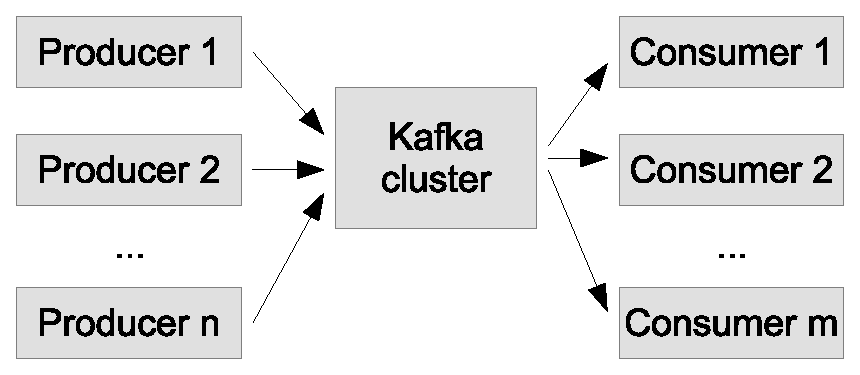
\includegraphics [width=0.5\textwidth]{images/kafka_structure}
  \caption{Kafka structure}
  \label{fig:kafka_structure}
\end{figure} 

\mnote{Kafka topic}
The core abstraction in Kafka is \textit{topic}.
One topic aggregates messages of one type.
For example, the system tracks the user activity, e.g. the number of times he opened a particular application or visited a particular website.
All these records are stored in the topic 'User activity'.
It is recommended to have a small number of topics (no more than a thousand).
However, each topic can contain  billions of messages.

One topic is a log that is spread over a cluster of brokers.
Every Kafka broker consists of zero or more partitions.
Figure~\ref{fig:kafka_topic_structure} illustrates the topic structure.
Kafka continually appends messages to the partitions.
Each partition represents an ordered sequence of messages that are uniquely identified by ids.
This id is called the \textit{offset}.
The sequence of messages is immutable and can only be extended by addition of new messages.
Besides appending, system provides one more operation: messages fetching.
Messages can be obtained from a particular partition, if a beginning message id is specified.
Kafka has an API for these operations, that can be used in different programming languages.

To provide fault tolerance, Kafka replicates each partition across several servers in a Kafka cluster.
One of these servers is a 'leader' and others are 'followers'.
The leader is responsible for handling all read and write requests.
The followers only replicate the leader.
For load balancing each server is simuntaneously a leader and a follower, i.e. for some of its partitions it acts as a leader and for others - as a follower.

The follower acts as a normal consumer, receiving data from the leader and applying it to its log.
Only when all the replicas received the message it is considered to be 'committed' and can be delivered to real consumers.
This guarantees that no message is lost even in the case of the leader failure.
A consumer always receives a message that is committed to the Kafka cluster.
A producer can wait until the message is committed or not, depending on the application logic.

To choose the leader, Kafka maintains a dynamic set of in-sync replicas (ISR).
Only these replicas can participate in the leader elections.
All these nodes must receive a message to consider it to be a committed write.
ZooKeeper stores the ISR set and tracks every change of its membership.
When a Kafka cluster has \textit{n}+1 replicas, it can sustain \textit{n} failures without any problems.

% �������� �������� ��� ��� � ������� ������ ����� ��� ���
%[reference: http://kafka.apache.org/documentation.html]
\begin{figure}[h]
  \centering
  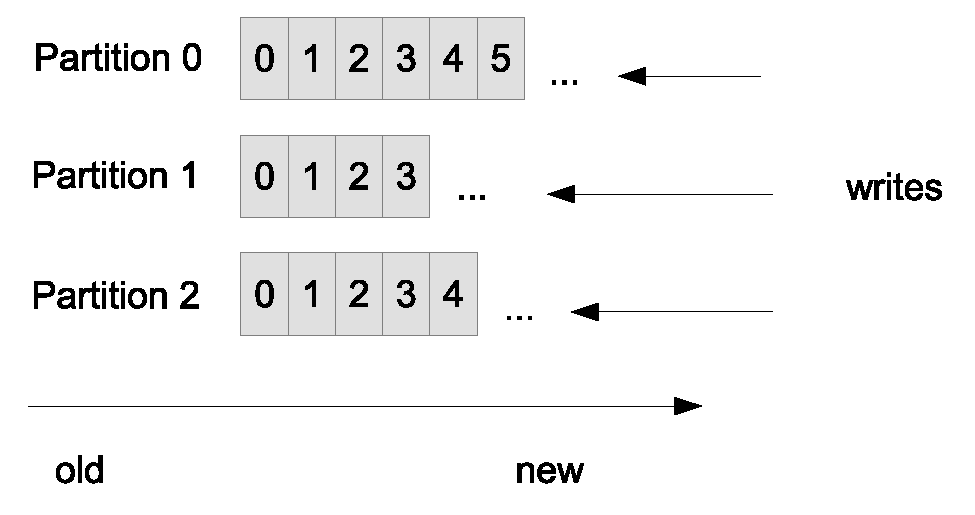
\includegraphics [width=0.5\textwidth]{images/kafka_topic_structure}
  \caption{Kafka topic structure}
  \label{fig:kafka_topic_structure}
\end{figure} 

Kafka uses a publish/subscribe mechanism to establish a communication process between producers and consumers of data.
One subscriber consists of a group of processes that run as a cluster.
Only one machine in this cluster obtains messages from Kafka.
Moreover, it consumes data from a specified partition.
Therefore, the subscriber parallelism depends on the number of partitions of the topic.
Kafka uses ZooKeeper to add or remove nodes from the broker and consumer groups.
It helps to rebalance the load automatically.

The fact that each partition has only one consumer makes it easier to store the metadata about what has been already consumed.
The consumer process just needs to store the last acknowledged message id.
Kafka uses 'at-least-once' semantic for message delivery.
It means that if the cunsumer process crashes, it reprocesses some messages from its partition one more time. 

There are two ways to balance load over Kafka brokers for message producers.
On the one hand, it can be done randomly.
On the other hand, application can supply a key that can be used to hash messages for partitioning.
The latter way guarantees the order of messages between partitions, that is not provided by Kafka.
Also it helps distributed consumers to make in-process aggregation.
In this case a consumer can obtain data from a particular partition, knowing that it contains a part of information it needs.  

For enhancing throughput Kafka introduces three techniques. 
First, it partitions data to production, consumption and brokering parts.
Second, it batches messages to chunks to send them together.
Third, it shrinks the data to decrease the amount of data that should be sent.

\mnote{batching}
The Kafka producer can send messages in synchronous or asynchronous ways.
In asynchronous mode small messages are collected into batches.
This allows to send data in chunks over the network. 
As it is done on application level, it is possible to control the batch size and the maximum time of holding the message.
Kafka allows to group messages from low-volume topics and high-volume topics together, reducing the amount of small requests.
On the filesystem level the mechanism of pagecache is used to buffer writes.
Kafka allows to delay the flush to disk again on the application level.
Similarly, it gives a control over the message boudaries and makes possible to have different policy for different topics.
Batching is also useful on the consumer side.
The client specifies the starting message id and the maximum buffer size it can receive at one time.
Kafka provides a possibility to combine data from several topics in one request.

\mnote{shrinking}
There are two techniques of data shrinking: via serialization and via compression.
Kafka associates schemas with the topics to extract the repeated structure from the messages.
Along with serialization, these schemas can be used to provide the compatibility and integration facilities.
The popular software that is used in combination with Kafka for serialization is Apache Avro.
It is described in details later in this chapter.
Kafka is able to compress several messages into a composite set of messages.
This is done during the batching process of the Kafka producer.
Thus, the messages in the compressed form are transferred to Kafka, where thay are stored and handled also in a compressed form. 

As the data transferred through Kafka is very diverse, a uniform schema is used for every topic.
This schema is kept all the way, from Kafka producer to Kafka consumer.
The schema usage is mandatory and is automatically checked.
As the schema sometimes changes, Kafka stores all its verions.
Each message contains a schema version id with which it was created.
Every schema is thoroughly tested when registered to detect incompatibilities in a timely manner.

\mnote{system monitoring}
A special Kafka topic exists to detect the percentage of data loss.
It audits the number of messages that are sent and received within a given topic over a specified period of time.
For this purpose each producer and consumer periodically notifies the audit topic about the number of processed messages.
The timestamps are extracted from the messages, instead of using the machine time of the message processing.
It is done to deal with delays in message delivering.
Kafka provides a standalone application for monitoring that processes the data from the audit topic.
It computes the ratio of data loss and duplication and is able to produce alert messages.

Kafka can by applied in a number of ways.
First, it can serve as a message broker, allowing to separate data producers from data processing.
Second, it provides facilities for real-time monitoring.
For instance, Kafka can be used to monitor the website users activity or to aggregate some application statistical data.
Third, it can serve as a log aggregation system, that can operate a log messages stream instead of dealing with log files.
This approach decreases latency and makes easier log data collection from several sources.

\mnote{log compaction}
One more Kafka application is a distributed system commit-log, that is used for restoring the failed nodes.
For this purpose Kafka has a specific feature - a \textit{log compaction}.
The main idea of log compaction is that Kafka guarantees that for all the message keys it retains the last known value.
The simpler data retention approaches are time- or size-based.
For example, Kafka removes the log data that is older than a specified period of time.
In this case some values that change rarely can be lost.
On the contrary, log compaction guarantees that at least the last value for each key persists.
This allows to fully restore the state of the broken node.

Another property of log compaction is that it shrinks the log size, removing the old records.
Using the complete log of all changes system can restore its state to any point by re-processing all the changes from the beginning of the log.
However, this approach requires a lot of memory for storing all the changes that leads to poor performance.
Log compaction removes only those records where more recent updates with the same key exist. 
Due to this fact the exterior system does not need to read the whole log and replay all the changes in order to restore its state.
Each topic has its own retention policy, i.e. one cluster can combine time or size retention with log compaction retention.

%[reference: http://kafka.apache.org/documentation.html#majordesignelements]
Figure~\ref{fig:kafka_log_structure} presents the Kafka log structure. 
The head of the log has a sequential numeration (offset) and retains all messages.
The tail of the log has a compacted structure, that contains only selected records.
It is important to mention that the messages in the log tail keep the original offset.
Kafka assignes this offset only once when a message is written for the first time and never changes it.
Moreover, even offsets for removed records are still valid log positions.
In this case Kafka returns the next highest existing value.
For instance, in our case requests with offsets 14, 15, 16 and 17 all return data starting from 17.

\begin{figure}[h]
  \centering
  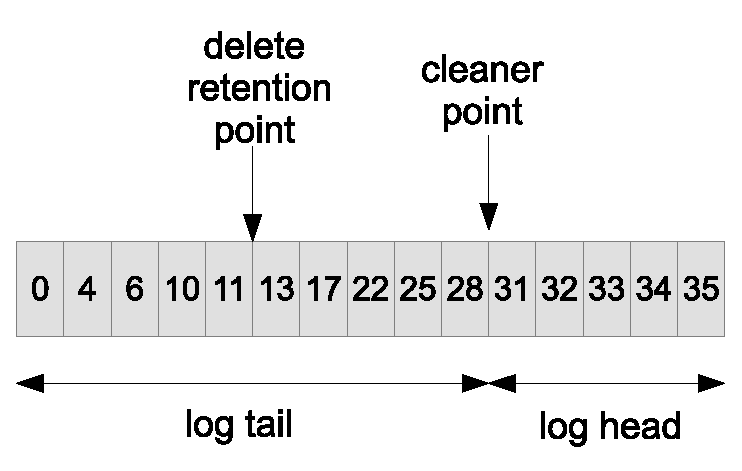
\includegraphics [width=0.5\textwidth]{images/kafka_log_structure}
  \caption{Kafka log structure}
  \label{fig:kafka_log_structure}
\end{figure} 

Compaction also performs message deletions.
If the message is marked to be deleted, all its previous versions (records with the same key) will be removed.
Deletion markers are not retained in the log after 'delete retention point' presented on the picture.

Log compaction is a background process that is run periodically.
Figure~\ref{fig:log_compaction_process} visualises a simple example.
Log compaction process posesses the following properties:
first, it guarantees the messages ordering even after compaction.
Second, the message offset is immutable and serves as a position of the record in the log.
Third, a read operation returns at least the final version for each value associated with a key.

\begin{figure}[h]
  \centering
  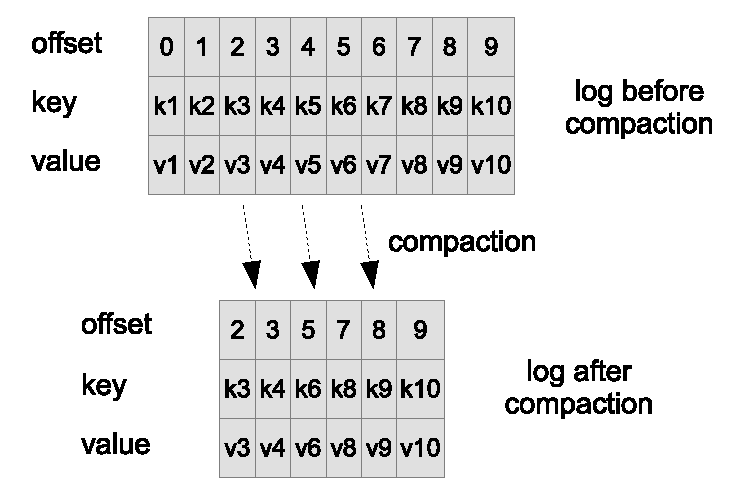
\includegraphics [width=0.6\textwidth]{images/log_compaction_process}
  \caption{Kafka log structure}
  \label{fig:log_compaction_process}
\end{figure} 

The compaction process consists of the following steps:
(1) The log is chosen, that has the biggest number of records from log head to log tail.
(2) For each key in the log head compaction process determines the last offset.
(3) The log is copied from the beginning to the end, removing the keys that occure later in the log. 
   



\subsection{RabbitMQ [VI]}

RabbitMQ is a queue messaging server \cite{RabbitMQ, AlvaroWilliams2012}.
It provides a robust, efficient and scalable message broker, that serves as an intermediate layer between sending and receiving clients.
RabbitMQ has a simple data model, that, nevertheless, offers a flexibility in the structure of data flows.
It gives an opportunity to adjust a tradeoff between throughput and reliability.
RabbitMQ fully applies Advanced Message Queuing Protocol (AMQP).

RabbitMQ is basically a delivery system, that receives messages, handles them, and then sends them to the destinations.
It is called also a \textit{broker server}\mnote{Broker server}.
It can serve messages coming from client apps to a server and backwards.
It also can be a mediator between client apps themselves.
RabbitMQ rules messages going through it, so that they are reliably stored, distributed, and then sent, possibly many times in case of absence of acknowledge from the destination.
It completely separates senders and receivers, so that they can be easily modified, removed, or added.
Figure~\ref{fig:RabbitMQGeneralStructure} shows general structure of RabbitMQ server and the flow of messages.

\begin{figure}[h]
  \centering
  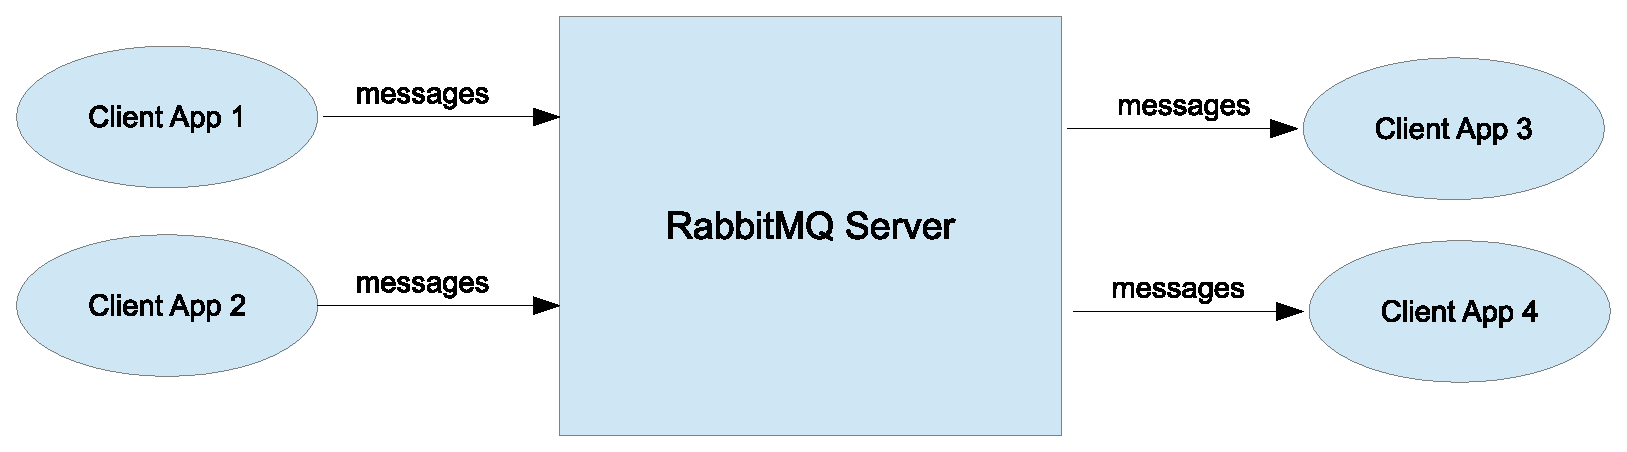
\includegraphics [width=0.9\textwidth]{images/RabbitMQGeneralStructure}
  \caption{General structure of RabbitMQ server and the flow of messages.}
  \label{fig:RabbitMQGeneralStructure}
\end{figure}

Client that sends messages is called \textit{producer}\mnote{Producer}.
Producer creates a message and sends (publishes) it to a broker.
Message consists of two parts: label and data.
Data can be anything, e.g. text, JSON object, JPG file, etc.
Label provides information about who should receive the message.
When producer sends a message, it does not wait for a confirmation from supposed receivers.
Such strategy is called fire-and-forget.
Broker acknowledges only the fact, that it has received the message properly.
It does not provide information to a sender about further life of the message. 

Client that receives messages is called \textit{consumer}\mnote{Consumer}.
Consumer subscribes to a specific \textit{queue} (we discuss queues in details below).
Broker transmits messages, coming to this queue, to all subscribed consumers.
There is no way to know who was a publisher of a message using label.
The only possibility is to sign this message inside of the data part, what is, basically, not in the scope of brokers's responsibilities.

The same application can be a producer and a consumer at the same time.
This is often a case, because application usually needs to communicate with the server or with other nodes of the network using broker server.
But it is important to mention, that there is, basically, no client and server notions in the discussed concept.
Rather it is a model of publishers and subscribers, or senders and receivers.
Broker server acts then as a middle transport layer.

For further discussion we need to describe \textit{Advanced Message Queuing Protocol} \mnote{Advanced Message Queuing Protocol (AMQP)} or \textit{AMQP} \cite{AMQP2011}.
AMQP is a protocol, that specifies common rules for messaging, queuing, publication/subscription, routing, etc.
It provides reliable, efficient, flexible, generic mechanisms for communication between clients.
AMQP is a binary protocol.
It has a set of commands, that must be implemented, e.g. \lstinline{open}, \lstinline{begin}, \lstinline{attach}, \lstinline{transfer}, \lstinline{flow}, \lstinline{disposition}, \lstinline{detach}, \lstinline{end}, \lstinline{close}.

In order to start publishing messages producer has first to connect to a broker.
It establishes TCP connection, and initializes \textit{AMQP channel} \mnote{AMQP channel} on top of it.
Such channel is only a virtual connection.
Producer can create many AMQP channels in parallel using one TCP connection.
This is useful, when for example one application needs to send many messages to the server from different threads.
It would be then very expensive to establish separate TCP connection for every thread.

Another important element of RabbitMQ broker server is Queue\mnote{Queue}.
It stores messages that are still not delivered.
Also, queue is a named object, and the name is an identifier for consumers, that want to subscribe to this queue.
There are two ways for a consumer to receive a message from the queue.
The first one is to subscribe to a queue and receive all messages that comes in it automatically.
This creates an AMQP channel, that is then used during the whole time of listening.
The second one is to retrieve a single message from a queue.
Consumer acknowledges received message to a broker.
In some cases it can reject message, for example when an error during its processing occured.
It is then important to specify (rejecting the message), that message must be sent to this consumer once more.

Consumers and producers can create queues.
Consumer must be unsubscribed from any other queue, declaring a new one.
Creating a queue, the one who does it must specify its name (or say to a broker to put random one and return it).
The name is important for producers, that want to publish to this queue.
There are two parameters to mention, that can be also specified.
The queue can be declared as exclusive, what means that only creating consumer is allowed to listen from it.
Another propery is auto-deletion, that says to a server, that queue must be deleted after the last consumer unsubscribes from it.

\textit{Exchange} \mnote{Exchange} is a component of RabbitMQ broker server that completes the whole picture.
Exchange is a place to where producer sends a message.
It is then redirected using specific rules to a particular queue.
Those rules are called \textit{routing keys}\mnote{Routing keys}.
It is said, that queue is bounded to an exchange by a routing key.
Each message that producer sends to a broker, has a routing key in its label.
Broker server tries then to match it with its bindings, to put the message in a proper queue.

There are four types of exchanges in RabbitMQ: direct, fanout, topic and header.
The difference between them is in the routing algorithm.
\textit{Direct exchange} simply matches routing key with the queues' names.
The messages goes then to the corresponding queue, always to only one among existent.
In the broker server there is always a default direct exchange, but it is possible to create more in case of specific needs of a system.
\textit{Fanout exchange} puts a message to all queues bounded to it.
It is useful, when the message must cause several different reactions.
\textit{Topic exchange} allows to send messages from different sources to the same queue, and to send messages from one source to several queues.
It is the most flexible and powerful type of exchange.
Different interesting messaging scenarious can be realized via topic exchange.
\textit{Header exchange} is similar to direct exchange, but rarely used, and we do not discuss it here.

Important concept in RabbitMQ is \textit{virtual host}\mnote{Virtual host}.
It is, basically, a virtual machine inside RabbitMQ server, that serves as a separate brocker.
This concept allows to separate different systems having the one RabbitMQ server.
Each virtual host has its completely own set of exchanges, queues and bindings.
It is easy to move virtual host from one RabbitMQ server to another, without necessity to think about what belongs to which brocker.

RabbitMQ provides \textit{durability} \mnote{Durability} of brocker's structure and exisiting messages.
If a machine with the RabbitMQ server goes down, or brocker just crashes - all exchanges, queues and messages inside will be recovered after restart.
But this mechanism is off by default, and must be switched on, in case durability is important.
To achieve this for every exchange and queue should be set to true parameter \lstinline{durable}.
Also, every message must have a \textit{delivery mode} set to 2, what informs the brocker, that it must be persisted in case of crash.
Broker writes then all needed for recovering information to a persistency log file.
It is important to remember, that durability and persistency affect efficiency, that is why they are switched off by default.
\subsection{Avro [SP]}
\label{subs:avro}

Data should be structured when it is transferred over the network.
Data objects are converted into some form, in which they can be stored or transferred and later be reconstructed in a new environment.
This process is called serialization.
The naive serialization approaches are XML or JSON.
Drawbacks of these formats that they require too much space for storing, because the data is kept it a text form.
The better solution is to use binary format for serialization and Apache Avro is one of the frameworks that use such approach.

Avro differs from the other serialization frameworks in that it does not require the code generation on receivivg.
It even allows to efficiently sort binary-encoded data without deserialization.
Also Avro supports easy schema changes, because it stores both old and new schemas and can associate fields with each other using their names.
This framework provides two types of encoding: binary encoding and using JSON.

Avro uses \textit{schemas} that are defined using JSON.
It needs a schema for serialization and in most cases this schema is transmitted along with the data.
Thus the receiving application does not need to store schemas for deserialization.
However, in some scenarios the transmission of schema is redundant, because both sides have the full schema stored locally.
In this case it is possible to transmitt only a binary representation of serialized objects.

The schema can contain both primitive and complex types.
Primitive types include: \textit{null}, \textit{boolean}, \textit{bytes}, \textit{int}, \textit{long}, \textit{string}, \textit{float} and \textit{double}.
Complex types are: \textit{record}, \textit{array}, \textit{enum}, \textit{union}, \textit{map} and \textit{fixed}.
Listing~\ref{lis:example_avro_schema} illustrates the example schema.
One schema files stores only one schema definition.

\begin{lstlisting}[caption=Avro schema (example), label=lis:example_avro_schema]
{
  "name":"AppInstall",
  "namespace": "example.avro",
  "type":"record",
  "fields":[
     { "name":"id", "type":"long" },
     { "name":"userId", "type":"long" },
     { "name":"time", "type":"long" },
     { "name":"appName", "type":"string" },
     { "name":"packageName", "type":"string" }
  ]
}
\end{lstlisting}

Avro uses an \textit{object container format} for storing objects in a file.
A file has a specified schema, that consists of blocks with synchronization markers between them.
Blocks contain data objects and can be compressed.
Synchronization markers allow to split file for processing it with MapReduce.
Moreover, Avro file comtains metadata section, where it stores a schema.

A file has the following structure: it has a header and one or several file data blocks.
The header contains information about encoding type and file metadata.
Metadata stores the schema and a type of codec that is used for compressing.
'null' codec type means that the data is uncompressed, 'deflate' codec uses the deflate algorithm.
The file data block stores information about the number of objects it contains, their sizes in bytes after compression, the serialized objects themselves and a synchronization marker.
This additional data helps to detect corrupted blocks.

Avro provides a \textit{Remote Procedure Call} (RPC) interface for implementing data exchange between a server and a client.
RPC protocol is defined using JSON.
Its attributes include a \textit{messages} object, that specifies the messages that are exchanged.  
\textit{Message} is a byte sequence, that is transmitted using a transport mechanism.
Transport system sends requests and receives responces.

Transport can have a stateless or stateful design.
\textit{Stateless} means that a server does not store any information about a client state.
The client transmitts all the needed data in every request message.
In \textit{stateful} design the server keeps the persistent client state.
This approaches has two problems.
First, the server should have a mechanism to discard client state at some point.
It is not possible to store the states of all the client for unlimited period of time.
Second, the server should be able to restore the client state in the case of the server crash.
This makes the process of server-side implementation complex comparing to sateless design.
However, stateful design results in better performance.
Figure~\ref{fig:stateful_stateless} represents the stateful and stateless schemas.

\begin{figure}
  \centering
  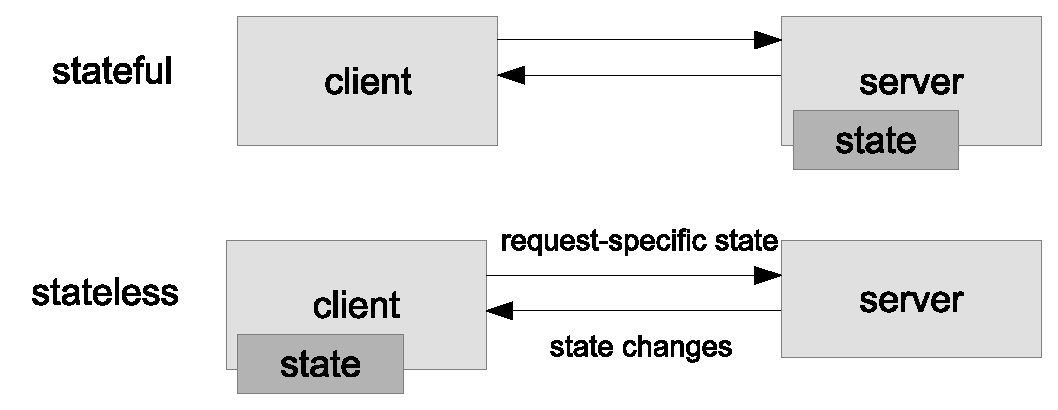
\includegraphics [width=0.7\textwidth]{images/stateful_stateless}
  \caption{Stateless and stateful design}
  \label{fig:stateful_stateless}
\end{figure}

An example of stateless transport method for Avro is HTTP.
In this case all Avro messages share the same URL at an HTTP server.
The 200 (OK) response code should be used by all response messages (normal and error).
Avro sends requests via the POST method.

There is an intermediate layer between messages and transport named \textit{framing}.
The main idea of framing is the partition of each message to a list of buffers.
A buffer contains buffer length followed by buffer data of this length.
Every message consists of one or several buffers.
Framing makes read and write operations more efficient.

Avro uses a handshake procedure before sending any RPC requests and responses.
It is used to make sure that the protocol definition is the same on both the server and the client side.
Only in this case the server and the client can correctly deserialize requests and responces.
To avoid extra network exchanges the server and the client stores recently used protocols in a cache.
Stateless and stateful transport differs in that the former requres a handshake before every request and response.
In contrast, the latter needs only one handshake and for the lifetime of the connection.

The handshake procedure is the following.
The client sends a \textit{HandshakeRequest} in a form \textit{(clientHash=clienthash, clientProtocol=null, serverHash=serverhash)}.
The \textit{clienthash} and the \textit{serverhash} are both the JSON protocol text, hashed with MD5.
The \textit{serverhash} contains data that the client received from the server during the last session.
If it is the first connection to this server the client tries to guess the server's hash.
The server sends in response a \textit{HandshakeResponse}.
If the received \textit{serverhash} is valid and the server knows the corresponding protocol to this client, the response has a form \textit{(match=BOTH, serverProtocol=null, serverHash=null)}.
In this case the connection is confirmed and the server can send a response message.
If the \textit{serverhash} is not valid, but the server knows the client protocol, it answers with \textit{(match=CLIENT, serverProtocol=serverprotocol, serverHash=serverhash)}.
It also allows the server to send the response data to the client.
However, the client must replace its nonvalid \textit{serverhash} data with that received from the server and process the response using the received protocol.
When the server is not aware of the client's protocol it received, it response with \textit{(match=NONE)}. 
Then the client re-sends its request extended by \textit{clientProtocol} value and the server response with \textit{(match=BOTH)}.

To determine the identity of the schemas stored on the client and the server side, Avro uses \textit{Parsing Canonical Form}.
It is a transformation, that removes data, irrelevant for the comparison, and normalizes the JSON text.
This canonical form can be used to create a fingerprint (an integer that serves as a unique id for a schema). 

 


\subsection{Thrift [VI]}
\label{subs:thrift}

Thrift is a framework for communication between different languages \cite{Slee2007, Thrift}.
It extracts parts of languages, that require the most usage in the interprocess interaction.
Thrift provides all basic data types, that are common for most of languages.
It separates data representation, transportation, and processing of input and output streams from each other.
Thrift has code generation tools, that produce code for all supported languages having once written definition of communication in Thrift.

Thrift has been developed at Facebook, as a result of a demand in a simple, high-performance bridge between different languages.
Solutions that were present before were too slow and clumsy, or just too limited in data types and communication needs.
Facebook had several requirements to Thrift, that it fulfilled in the implementation.
The first one is the common data type system, that saves programmer from using specific Trift data type or from writing specific serialization.
The second is transport mechanism, that separates data exchange from other layers of the program.
Next is a protocol, that defines how data is serialized to be transported.
Versioning, that allows to alter data structures or add arguments to functions without interrupting functioning of the system.
Processing of data streams, that is responsible for management of raw data, coming from the input stream, or going to the output stream. 

Thrift has a \textit{type} \mnote{Types} system, that allows programmer to code in native data types of the language, he uses.
It also saves him from writing any kind of serialization of his data structures or classes for transportation.
The Thrift IDL (Interface Definition Language) allows to describe in a file all data structures, that are to use in the interaction with another program, in a clear and compact way.
Thrift's type system contains only common types, that exist in almost any programming language.
The base types are: \lstinline{bool}, \lstinline{byte}, \lstinline{i16}, \lstinline{i32}, \lstinline{i64}, \lstinline{double}, \lstinline{string}.
All integer types are signed integers.
Facebook's developers decided, that there is no much use of unsigned integer.
They are always converted to signed integers in arithmetic operations.
Also there are languages, that do not support them at all.

Thrift supports four complex structures to define: structs, containers, exceptions and services.
\textit{Struct} corresponds basically to a class in any object-oriented language.
It allows to define indexed fields with default values.
In general, notation of structs is similar to a C struct definition.
\textit{Containers} correspond to commonly used containers in all languages, namely \lstinline{list<type>}, \lstinline{set<type>}, and \lstinline{map<type1, type2>}.
For example, in Java their mappings are \lstinline{ArrayList}, \lstinline{HashSet} and \lstinline{HashMap}, correspondingly.
The type of a container's element can be any supported type of Thrift, including structs and other containers.
\textit{Exceptions} are essentially the same as structs, but they derive base exception class in each particular language.
\textit{Sevices} correspond to interfaces or abstract classes (pure virtual class in C++) in programming languages.
Listing~\ref{listing:ThriftStructures} shows examples of notations of these Thrift's components.
Listings are taken from \cite{Slee2007} and modified.

\begin{lstlisting}[float=h, caption=Notation of Thrift's data structures., label=listing:ThriftStructures]
struct Example
{
	1:i32 number=10,
	2:i64 bigNumber,
	3:double decimals,
	4:string name="thrifty",
	5:list<i32> listOfVals,
	6:map<string, list<i32>> combinedMap
}
service StringCache
{
	void set(1:i32 key, 2:string value),
	string get(1:i32 key) throws (1:KeyNotFound knf),
	void delete(1:i32 key)
}
\end{lstlisting}

\textit{Transport} \mnote{Transport} layer in Thrift is responsible for managing data transportation issues.
It does not specify exact transport protocol or method, rather it provides common interface.
For example it can define a communication using network socket, or writing to a file or database.
Basically transport requires only to know how to read write data, and does not need to know the source and the destination.
The main methods of the transport interface are: \lstinline{open}, \lstinline{close}, \lstinline{isOpen}, \lstinline{read}, \lstinline{write}, \lstinline{flush}.
There are several implementations of Thrift's transport interface, namely \lstinline{TSocket} for TCP/IP communication, \lstinline{TFileTransport} for writing to the file, \lstinline{TMemoryBuffer} that allows to read and write directly to memory allocated for the process.

\textit{Protocol} \mnote{Protocol} layer in Thrift separates data representation and transportation.
It provides specific structure of messaging, but it need not to be aware about how data is encoded, as XML, ASCII or binary format.
Data only must to support a set of operations defined by a protocol's interface.

Interface of Thrift's protocol contains two types of methods: for messaging and for encoding particular types of data and structures.
It has many methods, several examples are: \lstinline{writeMessageBegin(name, type, seq)}, \lstinline{writeMessageEnd()}, \lstinline{writeStructBegin(name)}, \lstinline{writeStructEnd()}, \lstinline{writeFieldBegin(name, type, id)}, \lstinline{writeFieldEnd()}, \lstinline{writeBool(bool)}, \lstinline{writeI32(i32)}, \lstinline{writeDouble(double)}, \lstinline{writeString(string)}.
There are similar reading methods, that we omit here for conciseness.
Basically, every writing function has it reading pair.
Thrift supports streaming writing of data, that allows to write and read data simultaneously.
For this sake each field of a structure contains its type identifier, what allows to write/send the value as an atomic element to the stream.
Facebook has implemented for its needs an efficient binary format, that is in use in many of its backend services.

Thrift has a \textit{versioning} \mnote{Versioning} model, that allows to change and improve data structures and interfaces, and read old data without special additional adjustments.
To provide this feature, Thrift uses identifiers for fields and methods' arguments.
Each field in the structure has then a field that is unique.
On deserialization, generated code recognizes old fields and simply omits them.
For the case, when there is no expected field, Thrift provides each structure with a so called \lstinline{isset} object.
It specifies for each field whether it is present in the structure.
Reading the structure, it is always explicitly to check \lstinline{isset} for a particular field to read.
Protocol and transport interfaces of Thrift also support versioning, so that developer can change them to fit better his needs.
Listing~\ref{listing:ThriftIsset} shows an example of \lstinline{isset} structure.

\begin{lstlisting}[float=h, caption=Example of isset structure., label=listing:ThriftIsset]
class Example
{
	public:
		Example() :	number(10),	bigNumber(0), decimals(0) {}
		int32_t number;
		int64_t bigNumber;
		double decimals;
		struct __isset
		{
			__isset() :	number(false), bigNumber(false), decimals(false) {}
			bool number;
			bool bigNumber;
			bool decimals;
		} __isset;
...
}
\end{lstlisting}

%Case Analysis
%Protocol/Transport Versioning

Thrift provides \textit{RPC} \mnote{RPC} using interface \lstinline{TProcessor}.
The ides is to divide complex systems into many simple communicating elements, that works with inputs and outputs.
In most case it is only one input and one output that are to handle.
On the Listing~\ref{listing:ThriftTProcessor} is an interface of the \lstinline{TProcessor}.

\begin{lstlisting}[float=h, caption=Thrift's TProcessor interface., label=listing:ThriftTProcessor]
interface TProcessor
{
	bool process(TProtocol in, TProtocol out)
		throws TException
}
\end{lstlisting}

%Generated Code
%TServer The Thrift core library has already implemented the \lstinline{TServer} abstraction.

Thrift's \textit{implementation} \mnote{Implementation details} supports many commonly used programming languages, e.g. Java, C++, Python, PHP, Ruby, etc.
Facebook deploys servers mostly using C++, Java and Python.
Apache web server uses Thrift to provide transparent communication between backend and frontend using \lstinline{THttpClient}.
Names of RPC methods in Thrift are sent as strings, what is though more bandwidth consuming, but ease implementation and matching of versions of interface definitions.

% more details about implementation

Facebook implemented many services using Thrift \mnote{Facebook Thrift Services}.
Facebook Search service uses Thrift for realization of the underlying protocol and transport layer.
Also Facebook Search service comprises components written on different languages.
Web-part implemented using PHP, search engine using fast C++, statistical and testing components using Python.
All these components need to communicate in a fast, robust and simple way, and Thrift fulfils these properties.

\section{Real-time Data Processing Systems}

Efficient processing of big volumes of data is a crucial point for any big data system.
It must be easy to model, develop and maintain.
This section describes two data processing frameworks - \textit{Storm} and \textit{Spark}.
They have different computational models, but allow execution of the same computations.
The difference between them is that Storm is a truly real-time processing system, whereas Spark works essentially with batches, and has a streaming extension on top of batch computations.

\subsection{Storm [SP]}

Batch processing is not applicable for real time computing.
Hadoop, the best known tool for batch processing, is helpless when it is needed to handle streaming data and obtain immediate result.
The main advantage of real time processing, the guaranteed time delay between a request and a result can be broken simply because the waiting time for the next batch is too long.
Therefore new systems, designed for real-time processing, have appeared.
One of such systems is an open source project named \textit{Storm}.

Storm is a \textit{complex event-processing} (CEP) system.
Complex event processing means gathering data from different sources, combining it and making conclusions from it.
For example, such system keeps track of significant changes in traffic reports or stock market feeds and immediately responds to them. 

Storm is implemented in a dialect of the Lisp language named Clojure.
Clojure is a functional language like Lisp, but it also supports multithreaded programming.
Clojure runs on the Java Virtual Machine, however applications within Storm can be written in Java, Scala, JRuby, Perl and PHP.
Moreover, one can use a Structured Query Language adapter for streaming data directly into Storm topoloy.

\mnote{Storm architecture}
The Storm cluster has a master node called \textit{Nimbus} and \textit{worker} nodes.
Nimbus assignes tasks for workers and monitors failures.
There is a deamon called \textit{Supervisor} on every worker node.
The supervisor is responsible for starting and stopping worker processes assigned by Nimbus.
ZooKeeper coordinates the interaction between Nimbus and Supervisors.
It stores the state of all the nodes, making the system stable to failures.
If any of the nodes is killed, ZooKeeper immediately restarts it, enhancing Storm cluster stability.
ZooKeeper is described in more details later in this chapter.

The basic concept of Storm is a \textit{topology}.
It is a graph of computation, that shows how data should be processed and passed between the nodes.
One can implement a topology in any programming language, because topology definition is a Thrift structure.
Thrift is a framework that allows to develop cross-language services.	

The data stream consists of an unbounded set of \textit{tuples}.
A tuple can contain both standard data types (integer, float, byte array) as well as user-defined types.
Every stream has its own ID.
The sources of streams called \textit{spouts}. 

The next important Storm primitive is \textit{bolt}.
Figure~\ref{fig:storm_architecture} shows the interaction between spouts and bolts.
The stream of tuples originates from a spout and goes through a sequence of bolts.
Every bolt performs a transformation on incoming data stream, like aggregating, filtering, or interaction with external parts such as databases.
A bolt can receive information from several spouts and stream it to multiple bolts.

\begin{figure}
  \centering
  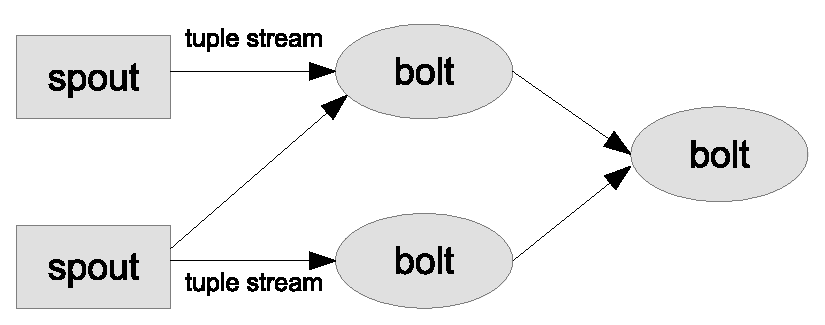
\includegraphics [width=0.5\textwidth]{images/storm_architecture}
  \caption{Storm architecture}
  \label{fig:storm_architecture}
\end{figure}

For example, MapReduce word counting example can be easily implemented with Storm.
Such system counts how many times each word occures in a given input data.
In the case of Storm one needs 
(1) a spout to generate text data, 
(2) one bolt to implement the Map function for word tokenisation and 
(3) one bolt to implement the Reduce function for aggregation the amounts of words occurences. 

Storm allows to group the stream of tuples in different ways.
For instance, shuffle grouping randomly distributes tuples to bolts such as each bolt receives approximately the same number of tuples.
Field grouping partitions tuples according to contained fields.
Also other grouping methods exist, including the custom grouping.

The Listing~\ref{lis:simple_storm_topology} represents a simple topology.

\begin{lstlisting}[caption=Simple Storm topology, label=lis:simple_storm_topology]
java TopologyBuilder builder = new TopologyBuilder();
builder.setSpout("myspout", new TestSpout(), 10);
builder.setBolt("mybolt1", new TestBolt(), 3) .shuffleGrouping("myspout");
builder.setBolt("mybolt2", new TestBolt(), 2) .shuffleGrouping("mybolt1");
\end{lstlisting}

Here topology consists of one spout and two bolts.
The stream of tuples originates from \textit{myspout}, then it is passed to \textit{mybolt1} and finally to \textit{mybolt2}.
In both cases tuples are grupped using the schuffle grouping method.
The integer numbers in \textit{setSpout} and \textit{setBolt} define the amount of parallelism for the node.

The implementation charasteristics of Storm lead to high performance and guaranteed fault tolerance.
It uses ZeroMQ for passing messages between the tasks.
Messages are automatically serialized and deserialized to Storm primitive types.
The usage of this message queue helps to avoid intermediate queueing, thus improving performance.
Furthermore, Storm guarantees the processing of every tuple.
In the case of a fault during message processing, a tuple is replayed from the spout.
There is also a fault detection mechanism on task level, when the failed task is quickly reassigned to restart the processing.
Storm has supervisors to manage the processes, that leads to efficient usage of resources.

Storm cooperates with message queue systems in such a way that every message is fully processed.
It builds a tuple tree, that reflects the motion af all the tuples.
Only when every message in the tuple tree is processed, a tuple is considered to be fully processed.

To give an example, let us take a message queue that supplies a spout with messages.
When the spout takes a message from the queue, the message state changes to 'pending'.
In this state it cannot be sent to other consumers.
Moreover, all the messages in pending state are returned to message queue if their consumer disconnects.
Storm assignes a unique id to the message, if it is not given by the message queue.
Using this id Storm can keep track of this message during processing.
The system receives this message when the \textit{nextTuple} method of the spout is called.
The spout emits the message along with its id to the consuming bolts.
When a tuple is fully processed, the \textit{ack} method of the original spout is called. 
In the case of time-out Storm calls the \textit{fail} method of the same spout.
Only when \textit{ack} or \textit{fail} method is called, the spout sends an ack or fail message to the message queue.
The message queue cancels the pending state of the message, taking it off the queue in the case of success and putting it back otherwise.

Storm can process not only the tuple trees, but also directed acyclic graphs.
It happens when an output tuple is anchored to several input tuples.
\textit{To anchor} means to specify a link in the tuple tree.
Multi-anchored tuples often appear during streaming aggregation or joining.
 
As it was mentioned, Storm tracks every tuple using its unique id.
Additionally, as each tuple exists within a tree, it knows all the tuples ids of this tree.
For example, if a bolt emits a new tuple, this tuple carries the ids of spout tuples received by this bolt along with its own id.
Such storage mechanism is used	because when the tuple is acked or failed, it should inform Storm about its dependencies to restore the state of the tuple tree.  

The acker task is responsible for acking the tuple.
First, Strom stores the mapping between an acker task and a spout tuple id.
As every tuple keeps ids of spout tuples in the tree it exists within, it knows the acker tasks it should communicate with.
A tuple informs an acker task when the tree is fully processed and the tuple is acked.
Second, the acker task should send a complition message to the spout task that emitted this tuple.
For this purpose, on creation of a new tuple a spout task notifies the appropriate acker task that its task id is linked to that spout tuple.

For acker task tracking the huge tuple trees explicitly is not efficient.
Thus Storm uses a special tracking strategy.
An acker task stores a map: on the one side it has a spout tuple id and on the other side a pair of values.
One of the values is a task id the spout tuple originates from, and the other is an 'ack val', the 64 bit number.
The 'ack val' represents the state of the tuple tree without storing it in memory.
This number is a result of XOR operation on all created and acked tuple ids of the tree.
Therefore, when the 'ack val' is equal to zero, it means that the tree is completed.
\subsection{Spark [VI]}

Spark is a framework for distributed processing of data \cite{Zaharia2010} \cite{Zaharia2013} \cite{Spark1} \cite{Spark2}.
It works with large datasets and streams of data, and lets to make complex queries on this data.
It consists of two parts: Spark engine that allows to process data in a batch fashion, and Spark streaming that extends Spark engine to handle fast coming streaming data.
Spark is simple, efficient and fault-tolerant.
It abstracts programmer from details of how processing distributes across cluster, and how robustness is achieved.
It shows results that surpass Hadoop in efficiency in 10 times.

Spark has several abstractions to represent data and streams.
Using them it is easy to write simple, short and robust code, that implements complex algorithms on batch and streaming data.
The first one - Resilient Distributed Dataset (RDD) - an object, distributed in the cluster, that contains data to process.
Another one is a Shared Variable - variable, that can be used among the cluster as a counter or a lookup table.
The last abstraction is a Discretized Stream (DStream) - representation of a data stream in a distributed fashion based on RDD objects.

%\subsubsection{Data model and batch processing}

\textit{Resilient Distributed Dataset} \mnote{Resilient Distributed Dataset} (RDD) is the main notion in Spark, that represents dataset in a distributed fashion.
RDD is essentially a readonly collection of elements.
It is fault-tolerant, so that if one partiotion is lost, the whole collection can be recovered.
RDD does not need to exist physically on the cluster nodes.
Instead, it is a lazy object, that can lay in a robust data storage, and be computed on the fly, when computations require particular pieces of data.
Figure~\ref{fig:RDDArchitecture} shows general architecture of an RDD object.

\begin{figure}[h]
  \centering
  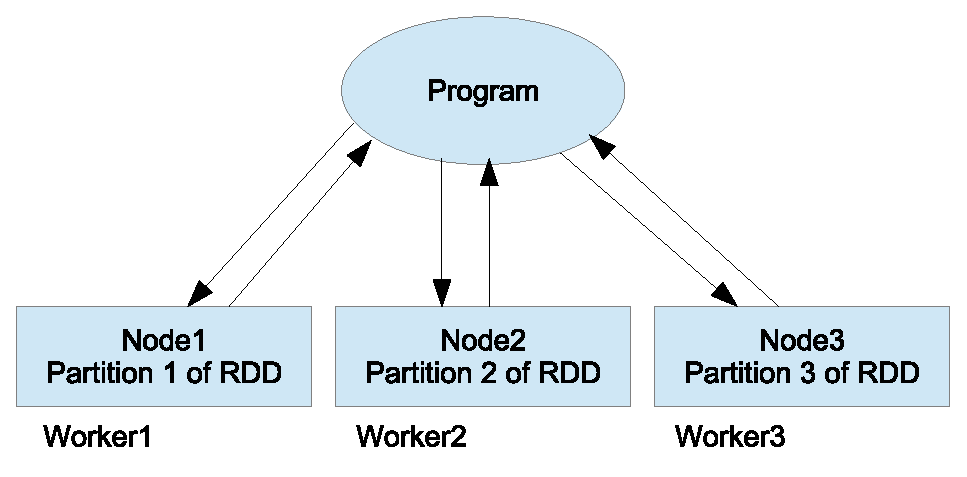
\includegraphics [width=0.7\textwidth]{images/RDDArchitecture}
  \caption{General architecture of an RDD object.}
  \label{fig:RDDArchitecture}
\end{figure}

There are two methods how to obtain an RDD object: parallelizing exisiting collection in the driver program, and using external dataset.
Existing collection is any collection of data, e.g. array, list, set, etc., that is directly handled in the program.
Creating an RDD object in this way, elements of a collection are copied to a distributed dataset, that can be used then in parallel.
It is possible to specify the number of slices, that is the number of tasks, each machine in the cluster will then execute for this collection.
External dataset is an external file.
It can reside in the local file system, and in the distributed file system like HDFS.
The simple example of processing data from the external text file in Spark, is to count the sum of lines' lengths using functions \lstinline{map} and \lstinline{reduce} of an RDD object. 
Additionally, it is possible to obtain RDD by transforming another RDD, or by changing persistance of an existing RDD, but this methods are derived in some sense.

RDD supports two types of operations: transformations and actions.
\textit{Trnsformation} \mnote{transformation} creates a new RDD object from existing one.
Examples of transformation are \lstinline{map}, \lstinline{flatMap}, \lstinline{filter}, \lstinline{groupByKey}, \lstinline{reduceByKey}.
For instance, a method \lstinline{map} processes each element of an RDD object using specified function, and returns a new RDD object as a result.
\textit{Action} \mnote{action} executes computations on an RDD object, and returns a value.
Examples of actions are \lstinline{reduce}, \lstinline{collect}, \lstinline{count}, \lstinline{countByKey}.
Method \lstinline{reduce} is a basic example of an action.
It aggregates all elements giving in the RDD object and return the resulting value.

Transformation in Spark is a lazy operation, in the sense that it is computed only when action operation requires its result to produce output.
This makes execution more efficient when there is a chain of transformations before final action, because the application does not receive then intermediate RDD objects, but only final resulting value, that is usually much smaller.
Nevertheless, there are cases, when it is to compute different actions on the same transformation.
Then it is meaningful to have RDD object of this transformation computed once, and to have a handle to it in the program.
For this case there is a method \lstinline{persist}, that allows to materialize RDD object.
This is also possible to persist RDD object on disk.

Fault-tolerance of Spark is based on HDFS and on the nature of RDD's realization.
As long as all data locates on HDFS, if any machine fails, all lost data can be recovered.
In case of node failure, RDD recovers itself, so that no data is lost, and processing is going without additional handling of administrator.

To initialize Spark it is first to create a \lstinline{SparkContext} object, that is responsible for a connection of the program to Spark.
It allows to specify properties of the application, and also options of how Spark should run, for example in local mode or on the cluster.
\lstinline{SparkContext} gives an access to different parameters and properties of execution environment.

\begin{lstlisting}[float=h, caption=Example of RDD usage., label=listing:RDDExampleCode, language=Java]
SparkConf conf =
		new SparkConf().setAppName(appName).setMaster(master);
JavaSparkContext sc = new JavaSparkContext(conf);
JavaRDD<String> lines = sc.textFile("data.txt");
JavaRDD<Integer> lineLengths = lines.map(s -> s.length());
int totalLength = lineLengths.reduce((a, b) -> a + b);
\end{lstlisting}

On the Listing~\ref{listing:RDDExampleCode} we present a simple program, that counts the sum length of all lines in the text file.
Example is taken from \cite{Spark1}.
Here we create an RDD object from external file, set \lstinline{map} function to count length of the each line, and set \lstinline{reduce} function to sum up lengths of lines.
Execution starts only when \lstinline{reduce} function is called, because, as we discussed, transformations are lazy in Spark.

Normally, passing arguments to a function, that executes on the nodes of the cluster, they are simply copied and there is no feedback to the driver program.
Sometimes it is useful to have global variable or lookup table, that all nodes can access.
Spark supports the notion of a \textit{shared variable}\mnote{shared variable}.
There are two types of shared variables: broadcast variables and accumulators.
\textit{Broadcast variable} \mnote{broadcast variable} represents readonly value or dataset, that is useful for all nodes as a lookup table or global predefined value.
It is copied to every node using method \lstinline{broadcast} of \lstinline{SparkContext}.
There are efficient algorithms in Spark to make this transfer fast.
\textit{Accumulator} \mnote{accumulator} is a distributed counter, that allows all nodes to add up to the global numeric variable.
It can be created using method \lstinline{accumulator} of \lstinline{SparkContext}.
No node can read this value or do anything else than incrementation, what makes its implementation easy and fast.
Only driver program is able to read accumulator's value.

%\subsubsection{Streaming processing}

\textit{Streaming in Spark} \mnote{Spark streaming} is an extension of a Spark engine, described in the previous section.
It can process data stream in a distributed manner.
Spark streaming receives data from the input stream, divides it into blocks, each represented as an RDD, and passes this sequence of blocks to the Spark engine.
It can work with different sources, e.g. message queue server (Kafka), web service (Twitter API), or regular TCP socket.
Processed data can be there stored to the filesystem or database.
The main abstraction for streaming processing in Spark is a Discretized Stream or DStream.
It is internally a sequence of RDDs.
Several DStreams can be combined into one chain for application more complex algorithms. 

\textit{Discretized Stream} or \textit{DStream} \mnote{Discretized Stream (DStream)} is the main abstraction in Spark streaming.
DStream can be the input stream, as well as intermediate stream, generated after processing of input stream of data.
It is essentially a chain of RDD objects, and provides a stream of data, that is to process by Spark.
Each RDD represents batch of data in the period of time, that is specified in the \lstinline{SparkStreamingContext}.
Figure~\ref{fig:SimpleDStream} depicts simple DStream.

\begin{figure}[h]
  \centering
  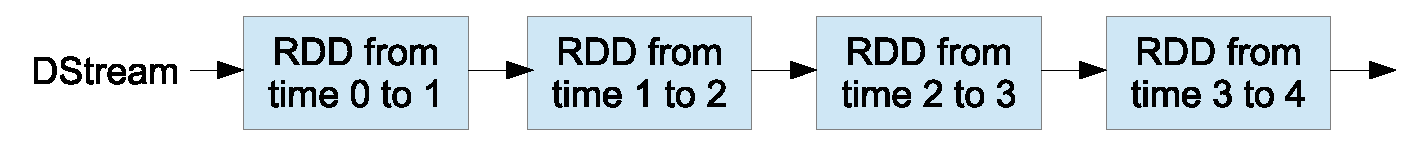
\includegraphics [width=1.0\textwidth]{images/SimpleDStream}
  \caption{Representation of a simple DStream.}
  \label{fig:SimpleDStream}
\end{figure}

Every operation, applied to DStream, is applied to every RDD object in the stream.
This implies, that transformation on the DStream produces new DStream.
All these transformations are executed by Spark engine in a standard batch fashion.
Figure~\ref{fig:DStreamWithTransformation} depicts how it works.

\begin{figure}[h]
  \centering
  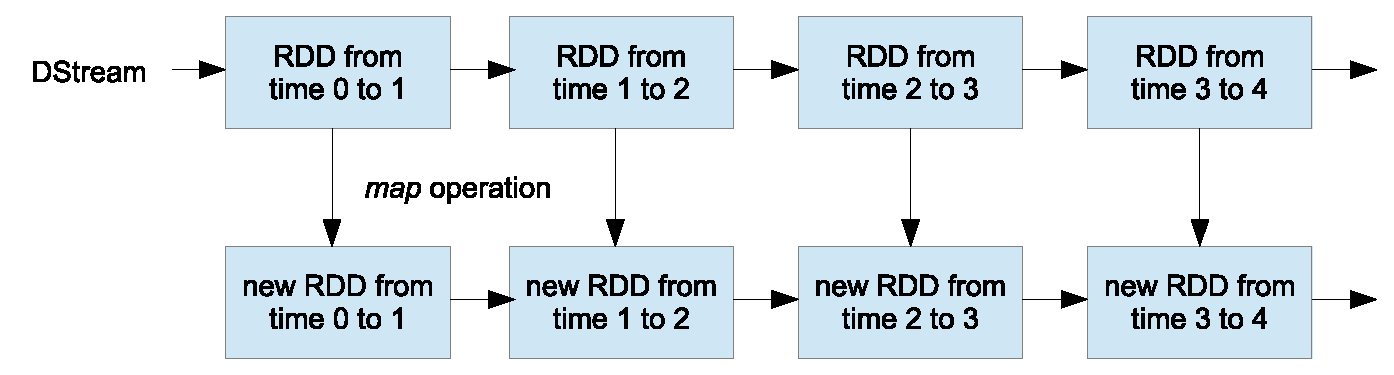
\includegraphics [width=1.0\textwidth]{images/DStreamWithTransformation}
  \caption{Transformation of a DStream to a new DStream.}
  \label{fig:DStreamWithTransformation}
\end{figure}

\textit{Input DStream} is a stream of raw data coming to Spark from the outer source.
Sources can be of two types: basic sources and advanced sources.
Basic sources are sources, that available using standard streaming context API, e.g. files or sockets.
Advanced sources are available using specific libraries, for example Kafka message queue server.
There is a notion of \lstinline{Receiver}, that is an object that receives data from the stream, put into Spark's memory, so that it is available for input DStream, associated with this Receiver.
Every DStream is responsible only for one input data stream.
Many DStreams can be created for different input streams to receive data from different data sources in parallel.
Receiver is executing as a long running task, hence it occupies one core of the processor.
This implies, that there should be more cores then receivers in the system.

There is a list of transformation to apply on a DStream.
They all are almost the same as transformations available for RDD, because DStream works on top of RDD.
The most common are \lstinline{map}, \lstinline{flatMap}, \lstinline{filter}, \lstinline{reduce}, \lstinline{reduceByKey}.

Similarly to Spark engine, it is to create \lstinline{SparkStreamingContext} object to work with Spark streaming.
It allows to adjust environment for processing, set properties like local or cluster mode, number of threads used, and many others.
One important property is the batch interval.
It defines the time of gathering data from the input stream, before creating RDD object and sending it to the Spark engine.

% must check this example
\begin{lstlisting}[float=h, caption=Example of DStream usage., label=listing:DStreamExampleCode, language=Java]
SparkConf conf = new SparkConf()
		.setMaster("local[2]").setAppName("NetworkWordCount");
JavaStreamingContext jssc =
		new JavaStreamingContext(conf, new Duration(1000));
JavaReceiverInputDStream<String> lines =
		jssc.socketTextStream("localhost", 9999);
JavaDStream<String> words =
		lines.flatMap(line -> Arrays.asList(line.split(" ")));
JavaPairDStream<String, Integer> pairs =
		words.map(w -> new Tuple2<String, Integer>(w, 1));
JavaPairDStream<String, Integer> wordCounts =
		pairs.reduceByKey((x, y) -> x + y);
wordCounts.print();
jssc.start();
jssc.awaitTermination();
\end{lstlisting}

Listing~\ref{listing:DStreamExampleCode} shows a simple example of a Spark streaming program.
Example is taken from \cite{Spark2}.
This code counts frequencies of words coming in a text data from the TCP socket.
First we create \lstinline{SparkStreamingContext} object, and specify it to work in a local mode using two execution threads.
We set a duration of gathering data from the input stream to 1 second.
In the line 3 we create DStream responsible for an input stream associated with TCP socket.
Then we apply two transformations and one action.
Transformations are \lstinline{map}-functions, so that the first one splits lines to words, and the second transforms words to pairs of the form \lstinline{(word, 1)}.
Action is a \lstinline{reduce} operation that sums up occurances of the same word.
Execution starts only when we call \lstinline{start} method of \lstinline{SparkStreamingContext}.
In the 7th line we print out partial results of the processing.
Instead, we can push results to a database or to a file, what is usually a case.

Spark streaming has a number of output operations on DStreams, that used to push transformed data to outer systems.
This can be files or databases.
Output operations actually start execution, as \lstinline{actions} of Spark engine do.
Examples of output operations are \lstinline{print}, \lstinline{saveAsObjectFiles}, \lstinline{saveAsTextFiles}, \lstinline{saveAsHadoopFiles}, \lstinline{foreachRDD}.

DStream allows to persist it in the memory, when multiple computations of the same DStream are required.
Method \lstinline{persist} of DStream object does that.
Its execution specifies that every RDD of the DStream will be persisted in the memory, as it is done for RDD in Spark engine.
For data, arriving from network, the persistence level is so, that all data is replicated to two nodes to provide fault-tolerance.

There is a mechanism of checkpointing in Spark streaming.
It allows to make snapshots of intermediate data to HDFS.
It makes computation throughput less, if set not properly.
So it must be carefully tuned.

\section{Storage Systems}

There are nowadays many different storage systems for big data management.
They have different data models and, hence, different applications.
Often they store data in a key-value manner.
In this section we consider three systems that are relevant for our work.
HDFS is a distributed file system that keeps data essentially in a tree structure in files.
Redis is a very simple in-memory key-value store.
Cassandra is more sophisticated column-style fully distributed data storage.

\subsection{HDFS [VI]}


\subsection{Redis [VI]}
\label{subs:redis}

Redis is an in-memory storage, that keeps data in a key-value fashion \cite{Seguin2012, Redis}.
It maintains data handled by a single application or by a cluster.
Redis is easy to deploy, learn and use.
It provides 5 data types, e.g. string, list, set, ordered set and hash, that are useful for different tasks, and give a powerful tool in combination.
Redis is an open source database system.

%\subsubsection{Basics}

Redis allows to create many different databases and switch between them.
Within one database Redis maintains a global map of keys to values.
The key is always a string.
It identifies piece of data, and does not represent data itself.

Redis provides many useful and simple commands to work with data.
The two simplest commands are \lstinline{SET} and \lstinline{GET}, that let to store a key-value pair into database, and to get value by key, respectively.
Listing~\ref{listing:RedisSetGet} shows an example of how to use these commands.
In this example the key is \lstinline{server:name} and the value is \lstinline{"SERVER1"}.

\begin{lstlisting}[float=h, caption=Example of usage of commands SET and GET., label=listing:RedisSetGet]
> SET server:name "SERVER1"
OK
> GET server:name
"SERVER1"
\end{lstlisting}

Redis allows to query values only by keys.
This is opposite to relational databases, where it is possible to search everything stored.
There is one exception, a command \lstinline{KEYS}, that returns all keys, stored in the database.
But it is strongly advised not to use it in production release, because it does a linear scan through all the keys, what can be very slow.
This command is rather for administrative issues.
Another point is that operation of receiving a value by a key works in a constant time, basically instantly.
This makes Redis in fact fast and useful, because grow of the database does not affect its performance.

Although Redis is an in-memory database system, it swaps data continuously to disk to provide persistance in case of application's failure.
Redis stores the database to disk every minute if at least 1000 keys have been changed.
It makes less swaps, if less keys have been changed.
It does swap completely as a snapshot.
There is though an alternative way to set Redis to make appending swaps.

%!!!!!!!!!!!!!!!!!!!!!!!!!!!!!
%Replications (can be written)
%!!!!!!!!!!!!!!!!!!!!!!!!!!!!!

%\subsubsection{Data types}

The basic data type in Redis is \textit{String}.
Keys are always strings.
Values can be of any type, but String is the most popular, because it represents atomic piece of data.
As a String it is possible to store not just something simple like name of a user or text data, but also complex objects like JSON object.
On the Listing~\ref{listing:RedisSETComplexValue} is an example of such action.

\begin{lstlisting}[float=h, caption=Usage of SET command with complex value., label=listing:RedisSETComplexValue]
> SET users:user001 '{"firstname":"john", "lastname":"smith"}'
OK
> GET users:user001
"{\"firstname\":\"john\", \"lastname\":\"smith\"}"
\end{lstlisting}

Redis provides standard commands to work with strings, e.g. \lstinline{STRLEN}, \lstinline{GETRANGE}, \lstinline{APPEND}, etc.
Storing a numeric value as a string, it is possible to work with it as with integer.
Redis has several useful commands for this case, e.g. \lstinline{INCR}, \lstinline{INCRBY}, \lstinline{DECR}, \lstinline{DECRBY}, \lstinline{SETBIT}, \lstinline{GETBIT}.
On the Listing~\ref{listing:RedisIntegerValue} is an example of working with value as with integer.

\begin{lstlisting}[float=h, caption=Working with value as with integer., label=listing:RedisIntegerValue]
> SET x 1
OK
> INCR x
(integer) 2
> INCRBY x 5
(integer) 7
> DECR x
(integer) 6
> DECRBY x 3
(integer) 3
> GET x
"3"
\end{lstlisting}

The first complex data type in Redis is \textit{List}.
List is simply an array of values identified by a key.
There are specific commands to work with lists, e.g. \lstinline{LPUSH}, \lstinline{RPUSH}, \lstinline{LRANGE}, \lstinline{LLEN}, \lstinline{LPOP}, \lstinline{RPOP}, etc.
Values of the list can be anything, not only strings.
This gives powerful tool to store complex combined data.
Listing~\ref{listing:RedisListCommands} shows basic usage of Lists.

\begin{lstlisting}[float=h, caption=Usage of List data type commands., label=listing:RedisListCommands]
> LPUSH users john mike jack
(integer) 3
> LRANGE users 0 -1
1) "jack"
2) "mike"
3) "john"
\end{lstlisting}

The next data type is \textit{Set}.
Set is an unordered array of distinct values.
There are many useful operations to work with sets in Redis, e.g. \lstinline{SADD}, \lstinline{SISMEMBER}, \lstinline{SINTER}, \lstinline{SINTERSTORE}, etc.
Set is implemented internally as a hash-table, hence, it provides constant lookup.
Listing~\ref{listing:RedisSetCommands} shows basic usage of Sets.

\begin{lstlisting}[float=h, caption=Usage of Set data type commands., label=listing:RedisSetCommands]
> SADD friends:john mike paul jack tania
(integer) 4
> SISMEMBER friends:john paul
(integer) 1 
\end{lstlisting}

\textit{Sorted set} is an extension of a regular Set, that provides order for its elements.
To order values, it uses scores.
Each value has then a score, that must be set together with inserted value.
It is possible then to lookup all values in the specific range of the score, or obtain all values in the sorted order.
Main commands for working with Sorted sets are \lstinline{ZADD}, \lstinline{ZCOUNT}, \lstinline{ZRANK}, \lstinline{ZREVRANK}, etc.
In case when it is needed to get array sorted by integers, Sorted set is a perfect data structure to do that.
Listing~\ref{listing:RedisSortedSetCommands} shows basic usage of Sorted sets.

\begin{lstlisting}[float=h, caption=Usage of Sorted set data type commands., label=listing:RedisSortedSetCommands]
> ZADD friends:john 70 mike 95 paul 92 jack 75 tania 1 dave
(integer) 5
> ZCOUNT friends:john 90 100
(integer) 2
\end{lstlisting}

\textit{Hash} is the last data type given in Redis.
Hash is essentially a hash-table, that maps strings to any objects.
It works also in constant time.
There are different commands to work with Hashes, e.g. \lstinline{HSET}, \lstinline{GHET}, \lstinline{HMSET}, \lstinline{HMGET}, \lstinline{HGETALL}, \lstinline{HKEYS}, \lstinline{HDEL}, etc.
Hashes give simple useful tool to store objects in an object-oriented way.
For example, instead of storing information about user as a JSON object, or as another string representation, it can be done using Hash.
Every field of a user is then put as a separate key-value pair.
Listing~\ref{listing:RedisHashCommands} shows basic usage of Hashes.

\begin{lstlisting}[float=h, caption=Usage of Hash data type commands., label=listing:RedisHashCommands]
> HSET users:john id 375
(integer) 1
> HSET users:john name "john"
(integer) 1
> HSET users:john lastname "smith"
(integer) 1
> HGETALL users:john
1) "id"
2) "375"
3) "name"
4) "john"
5) "lastname"
6) "smith"
\end{lstlisting}

%\subsubsection{Features}

Redis allows to use transactions to make several operations atomic.
Basically, any single operation that Redis does, is atomic, because Redis is single-threaded server.
On execution of any single command, no other command can start execution before the first one is in progress.
But sometimes it is useful or even necessary to do several operations in line as one atomic command.
For that case Redis provides transactions.
Listing~\ref{listing:RedisMultiExec} shows usage of transactions.
All commands between \lstinline{MULTI} and \lstinline{EXEC} is one the atomic operation.

\begin{lstlisting}[float=h, caption=Usage of commands MULTI and EXEC., label=listing:RedisMultiExec]
MULTI
...
EXEC
\end{lstlisting}

Redis allows to set expiration time for a key, or set an expiration point in time using Unix timestamp.
This can be done using commands \lstinline{EXPIRE} and \lstinline{EXPIREAT}.
It does not important, what data structure a key identifies.
When a key expires, it does not exist in Redis anymore.
To check expiration time for a key there is a command \lstinline{TTL}.
To remove expiration from a key, command \lstinline{PERSIST} exists.
Listing~\ref{listing:RedisExpire} shows usage of commands for setting expiration time.

\begin{lstlisting}[float=h, caption=Usage of commands EXPIRE and EXPIREAT., label=listing:RedisExpire]
> SET user001 "john smith"
OK
> EXPIRE user001 60
(integer) 1
> EXPIREAT user001 14572436115
(integer) 1
\end{lstlisting}

There is a mechanism of subscribtion and publication in Redis.
To subscribe to a channel, command \lstinline{SUBSCRIBE} exists.
When somebody publishes something to this channel using command \lstinline{PUBLISH}, subscribers receive this message.
This tool allows to notify different nodes in the system, that connect to Redis database, about events.

Redis has a useful command \lstinline{SORT}, that allows to sort lists, sets and sorted sets by their values.
Applied to a collection, this command returns elements in a sorted order.
There are different parameters to inform this command how to execute sorting.
Listing~\ref{listing:RedisSort} shows a simple example of how to use command \lstinline{SORT}.

\begin{lstlisting}[float=h, caption=Usage of SORT command., label=listing:RedisSort]
> RPUSH simple_array 3 12 7 1 4 8 2 9
(integer) 8
> SORT simple_array
1) "1"
2) "2"
3) "3"
4) "4"
5) "7"
6) "8"
7) "9"
8) "12"
\end{lstlisting}

Redis allows to use Lua scripts.
It is possible to write a script, to store it, and then to use directly as any Redis command.
This feature gives an opportunity to write own commands, that contain several actions, logically united in one meaningful operation.
Such defined procedure executes in atomic way, what is another advantage.
\subsection{Cassandra [VI]}

Cassandra is a distributed storage system \cite{Cassandra, Avinash2014, Hewitt2011}.
It is efficient and reliable.
It keeps data on many commodity machines without having master node.
This leads to

CQL

General architecture
Cluster
Data center
Commit log
Table
SSTable

Internode communications (gossip)
Failure detection and recovery

Data distribution and replication
Consistent hashing
Virtual nodes
Data replication

Partitioners
Murmur3Partitioner
RandomPartitioner
ByteOrderedPartitioner

Snitches
Dynamic snitching
SimpleSnitch

Client requests

\section{Configuraion Management}

As long as we use many software elements in the system, it is necessary to manage a lot of configuration data.
ZooKeeper solves this task.

\subsection{ZooKeeper [SP]}

Large distributed systems require a coordinator for system configuration management.
As it was mentioned in Chapter 4, Google uses a Chubby service for this purpose.
The main Chubby disadvantage is that for lock and unlock operations it is necessary to open and close the object consequently.
This feature influences the performance, increasing the time needed for making a lock.
Therefore Yahoo developes its own service named ZooKeeper that manages systems configuration and allows to efficiently lock the shared resources.

ZooKeeper namespace looks similar to a standard file system.
It consists of interconnected nodes, each of them identified by a path.
The path contains elements separated by a slash ('/').
Like in a file system, every node except the root has a parent node.
The parent node's path is a prefix for the current node path.
The ZooKeeper namespace differs from a standard file system in that its node can be a file and a directory simultaneously.

There are two types of nodes: persistent and ephemeral.
ZooKeeper stores persistent nodes on the disk, while ephemeral nodes belong to a particular session and exist only during this session.
Ephemeral nodes cannot have children nodes, they can only store data.
ZooKeeper client establishes a session with a ZooKeeper server, passing heartbeat messages.
When a client stopes to receive heartbeat messages, it reconnects to a defferent server, reestablishing the session.
If the session is canceled, all its ephemeral nodes are automatically removed.
ZooKeeper tree is presented in Figure~\ref{fig:zookeeper_tree} where the dark nodes are ephemeral.

\begin{figure}
  \centering
  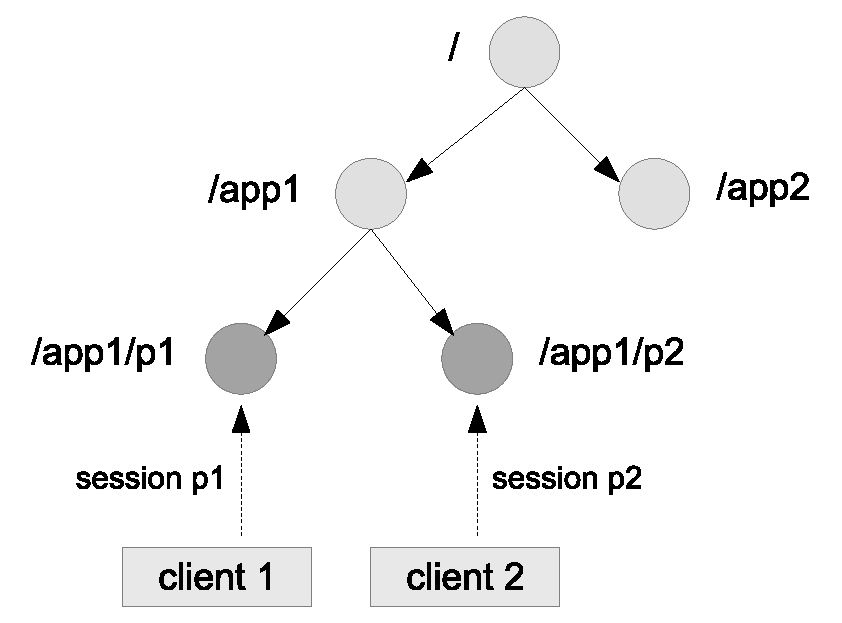
\includegraphics [width=0.5\textwidth]{images/zookeeper_tree}
  \caption{ZooKeeper tree sructure}
  \label{fig:zookeeper_tree}
\end{figure}

ZooKeeper is designed for small data warehousing, such as configuration, status and location information.
One node is usually not bigger than one kilobyte.
Therefore it stores data tree image in memory, keeping in a persistent store only transaction logs and snapshots.
In-memory storage limits the size of the database of ZooKeeper.
However, it gives advantages of low latency and high performance. 

The key feature of ZooKeeper is that it uses First In, First Out (FIFO) method for processing the messages.
It means that all commands are performed in the order they are received.
Thus, ZooKeeper maintains the total ordering.
The order is specified by a unique ZooKeeper Transaction id, that is assigned to each update.
 
ZooKeeper supports idempotent operations.
If a node should be updated, the system makes a note about the update and keeps an old and a new version of this node.
This allows client to receive the same message several times, being aware of when it can be applied.
Therefore all the write operations are performed sequentially in one thread and only on the master node.
On the contrary, read requests do not necessarily need the master node, they can be handled by a node's replica.

The client also supports the total ordering of the messages.
Hence if the client sends a write request and then a read request, the write operation is performed first.
Even if usually read operation does not need a lock, ZooKeeper strictly follows the order.
It allows to implement predictable asynchronous systems that work with ZooKeeper.

A client can watch a node.
If it sets a watch, it gets notified when the node is changed.
When the node sends this notification, it removes the watch.
In the case of connection problems between the client and the ZooKeeper server, the client receives a local notification.

ZooKeeper guarantees reliability using replication.
Its database is replicated to several nodes, one of them is a \textit{Leader} and the others are \textit{Followers}.
\textit{ZooKeeper Atomic Broadcast} (Zab) algorithm is used for managing the communication between the leader and the followers.
It synchronizes the replicas, broadcasts updates and recovers the valid state in the case of nodes crash.

Zab includes four phases: (1) Leader election, (2) Discovery, (3) Synchronization and (4) Broadcast.

1. On the first stage ZooKeeper uses any election algorithm to choose a leader.
After termination every node stores its vote locally in volatile memory.
When a node \textit{n} votes for a node \textit{n'}, \textit{n'} becomes a \textit{prospective leader} for \textit{n}.

2. On the second stage the nodes inform the prospective leader about the most recent transactions they accepted.
Thus the prospective leader knows the latest sequence af accepted transactions and can establish a new epoch.
From thit moment the previous leaders cannot perform any commits.
In the case of connection problems between a follower and a leader, the follower goes back to the stage (1) of this algorithm.

3. The leader is aware of the latests transactions history and during this stage synchronizes this information with its replicas.
This phase is also called voting phase, because it receives the votes from the nodes.
The leader performes a commit only if it receives acknowledgements from two of three followers.
At this moment the leader changes its state from \textit{prospective} to \textit{established}.

4. The nodes persist in this stage until a crash.
Every write request from a ZooKeeper client is broadcasted among the nodes.
New followers can join, receiving the transaction history from the leader.
The leader and its followers use periodic heartbeat messages for early failure detection.
If any of the nodes does nor receive a heartbeat message within a timeout, it shifts its state to \textit{election} and goes back to the first stage.

It can happened that one of the followers still has an outdated information when it receives the read request.
To avoid this problem, it is possible to make a force synchronisation with the master.
It is called the \textit{slow read}.
Evidently, if all the clients use the slow read the system looses the advantage of scaling.
Without force synchronisation ZooKeeper system scales for reads nicely. 
However, in this case the client that reads from a replica can obtain the outdated information.